% main.tex - Libro: Diseño de Experimentos en Ingeniería
\documentclass[compacto,10pt,comentarios]{aleph-notas}

% ===== CONFIGURACIÓN ADICIONAL =====
\usepackage{enumitem}
\usepackage{booktabs}
\usepackage{multirow}
\usepackage{array}
\usepackage{graphicx}
\usepackage{rotating}   % para \rotatebox
\usepackage{xcolor}     % para colores
\usepackage{pgfplots}   % para gráficas con axis
\usepackage{listings}   % para bloques de código
\pgfplotsset{compat=1.18}
\usepgfplotslibrary{statistics}
\lstset{basicstyle=\ttfamily\fontseries{m}\selectfont\small, columns=fullflexible}
\usepackage{booktabs}   % para líneas \toprule, \midrule, \bottomrule
\usepackage{array}      % para formato de columnas
\emergencystretch=2em
\hfuzz=12pt
\hbadness=10000
\newtcolorbox{observacion}{color=colordef,recuadrost}
\newtcolorbox{important}{color=yellow,postit}

% Personalización de colores (sobreescribe los de aleph-notas)
\definecolor{colorprincipal}{cmyk}{0.81,0.62,0.00,0.22}
\definecolor{colorsecundario}{RGB}{255,153,0}
\definecolor{colorejemplo}{RGB}{240,248,255}

% ===== DATOS DEL LIBRO =====
\institucion{Universidad Autónoma Metropolitana}
\asignatura{Diseño de Experimentos en Ingeniería}
\tema{Aprende Diseño de Experimentos desde la práctica y la vida cotidiana}
\autor{Roman Anselmo Mora-Gutiérrez}
\fecha{\today}
\fuente{montserrat}
\newcommand{\autoresproyecto}{%
Roman Anselmo Mora-Gutiérrez;
Edwin Montes-Orozco;
Eric Alfredo Rincón-García;
Sergio G. de-los-Cobos-Silva;
Pedro Lara-Velázquez;
Miguel Angel Gutiérrez-Andrade;
Gilberto Sinuhe Torres-Cockrell;
Isrrael Satiago Rubio;
Oswaldo Sanchez Andrade;
Oscar Antonio Manzanares Betancourt;
Yadira Alatriste Martínez;
Cesar Simon Lopez Monsalvo;
Luis Angel Meza Zarate}

% ===== LOGOS =====

% ===== INICIO DEL DOCUMENTO =====
\begin{document}

% ==================================================
% PORTADA PERSONALIZADA (antes del \encabezado)
% ==================================================
\begin{titlepage}
    \centering
    \vspace*{1cm}
    
    {\Huge\bfseries\color{colorprincipal} Diseño de Experimentos\par}
    {\huge en Ingeniería\par}
    \vspace{0.5cm}
    {\Large\textit{Aprende desde la práctica y la vida cotidiana}\par}
    \vspace{2cm}
    
    % Autores
    {\Large \textbf{Autores y colaboradores académicos}\par}
    \vspace{0.35cm}
    {\normalsize
    \begin{minipage}{0.86\textwidth}
    \centering
    \autoresproyecto
    \end{minipage}
    \par}
    \vspace{0.3cm}
    {\large Universidad Autónoma Metropolitana\par}
    \vspace{1cm}
    
    % Fecha
    {\large \today\par}
    \vfill
    
    % Línea decorativa
    \rule{0.8\textwidth}{0.5pt}
    \vspace{0.3cm}
    {\small Diseño de Experimentos en Ingeniería \textbullet{} Material didáctico \textbullet{} UAM}
\end{titlepage}

% ==================================================
% ENCABEZADO Y PÁGINA DE CRÉDITOS
% ==================================================
\encabezado

% Página de derechos reservados (opcional)
\newpage
\thispagestyle{empty}
\vspace*{\fill}
\begin{center}
    \small
    \textcopyright\ \today\ Roman Anselmo Mora-Gutiérrez \\
    Universidad Autónoma Metropolitana \\
    \vspace{0.5cm}
    Autores y colaboradores académicos considerados en el proyecto: \\
    \vspace{0.2cm}
    \begin{minipage}{0.86\textwidth}
    \centering
    \autoresproyecto
    \end{minipage}
    \vspace{0.6cm}

    Esta obra está bajo una licencia Creative Commons \\
    Atribución-NoComercial-CompartirIgual 4.0 Internacional.
\end{center}
\vspace*{1cm}
\newpage

% ==================================================
% DEDICATORIA (opcional)
% ==================================================
\newpage
\thispagestyle{empty}
\vspace*{\fill}
\begin{center}
    \itshape
    A mis estudiantes, \\
    porque aprender estadística también puede ser creativo y divertido.
\end{center}
\vspace*{\fill}
\newpage

% ==================================================
% ÍNDICES
% ==================================================

% Índice general
\tableofcontents
\newpage

% Índice de figuras
\listoffigures
\newpage

% Índice de tablas
\listoftables
\newpage

% ==================================================
% PRÓLOGO / INTRODUCCIÓN GENERAL
% ==================================================
% ==================================================
% CAPÍTULOS PRINCIPALES
% ==================================================
\section*{Ruta didáctica del manual}
\addcontentsline{toc}{section}{Ruta didáctica del manual}

Este manual no debe leerse como una colección de prácticas. Su propósito es acompañar al estudiante en una secuencia de decisiones experimentales: primero observar un fenómeno, después convertirlo en una pregunta, más tarde medirlo con cuidado y finalmente decidir con evidencia.

\begin{important}
La pregunta que guía el manual es simple: ¿cómo puede un ingeniero distinguir entre una impresión, una diferencia real y una conclusión defendible?
\end{important}

La lectura se organiza en cinco movimientos:

\begin{enumerate}
\item \textbf{Observar sin engañarse.} El estudiante comienza con fenómenos cotidianos y aprende que una sola observación no basta para afirmar una causa.
\item \textbf{Medir la variabilidad.} Antes de comparar tratamientos, se aprende a mirar muestras, medias, dispersión, datos faltantes y sesgos.
\item \textbf{Comparar tratamientos.} El ANOVA aparece como una forma de razonar con variabilidad, no como una tabla que se llena mecánicamente.
\item \textbf{Diseñar combinaciones.} Los diseños factoriales permiten estudiar factores, niveles, interacciones, blancos y réplicas.
\item \textbf{Decidir en sistemas reales.} Taguchi, modelos, ANCOVA, MANOVA y proyectos integradores se presentan como extensiones para problemas donde el experimento ideal no siempre es posible.
\end{enumerate}

Cada práctica debe cumplir una función dentro de esa ruta. Si una actividad no ayuda a formular mejor la pregunta, medir mejor, comparar mejor o decidir mejor, entonces debe reescribirse o moverse.

\begin{observacion}
Los documentos originales son materia prima. El estudiante no necesita saber de qué archivo provino una idea; necesita entender por qué aparece en ese momento del aprendizaje.
\end{observacion}

\newpage


\section{Gatos y grandes números: cómo el muestreo modifica nuestra percepción}

\subsection{Introducción}

¿Alguna vez te has preguntado cuántos gatos hay realmente dentro de la UAM?

La pregunta parece sencilla, pero cuando varias personas comenzaron a discutir el tema aparecieron respuestas muy distintas. Algunos compañeros aseguraban que casi nunca veían gatos, mientras que otros afirmaban encontrarse varios todos los días, especialmente cerca de Villa Miau o en algunas zonas tranquilas del campus.

Incluso aparecieron comentarios como:

\begin{quote}
“en las tardes salen más”
\end{quote}

o bien:

\begin{quote}
“cuando hay mucho ruido desaparecen”.
\end{quote}

En ese momento surgió una idea interesante: transformar una observación cotidiana en un pequeño experimento estadístico.

La intención inicial no era únicamente contar gatos. En realidad, queríamos observar cómo cambian:

\begin{itemize}
\item las frecuencias observadas,
\item la media,
\item la varianza,
\item y las probabilidades empíricas
\end{itemize}

conforme aumenta el número de observaciones.

En otras palabras, buscábamos entender experimentalmente cómo el tamaño de muestra modifica nuestra percepción de un fenómeno.

\subsection{Objetivo}

Analizar cómo el tamaño de muestra modifica el comportamiento de estadísticos como la media y la varianza mediante un muestreo empírico de gatos dentro de la UAM Azcapotzalco.

\subsection{Diseño metodológico}

El experimento se desarrolló utilizando observación pasiva. Durante el estudio no se alimentó ni alteró el comportamiento de los animales con el objetivo de evitar introducir sesgos externos en las observaciones.

Las observaciones se realizaron en distintas zonas de la UAM Azcapotzalco, incluyendo:

\begin{itemize}
\item Villa Miau,
\item pasillos del edificio E,
\item jardineras,
\item estacionamientos,
\item plazas abiertas,
\item y zonas cercanas a biblioteca.
\end{itemize}

\subsection{Control experimental y regla antiduplicación}

Uno de los problemas más importantes del experimento fue evitar contar dos veces al mismo gato.

Para disminuir este problema se estableció una regla antiduplicación basada en:

\begin{itemize}
\item color del pelaje,
\item tamaño,
\item manchas,
\item color de ojos,
\item y dirección de movimiento.
\end{itemize}

Además, en algunos muestreos se realizaron observaciones simultáneas en distintas zonas con el objetivo de disminuir la probabilidad de doble conteo.

\subsection{Homogeneización del tiempo de observación}

Todos los equipos acordaron trabajar utilizando periodos homogéneos de:

\[
\boxed{2 \text{ minutos por observación}}
\]

De esta manera, cada muestra representa:

\begin{center}
\textit{el número de gatos observados durante un periodo fijo de dos minutos.}
\end{center}

\subsection{Duración y tamaño de muestra}

Es importante aclarar que los valores:

\[
n = 2,\; 5,\; 10,\; 15,\; 20
\]

no representan tiempo, sino el número total de observaciones realizadas.

Cada valor de \(n\) corresponde al número de veces que se repitió el proceso de observación de 2 minutos.

\subsection{Resultados experimentales: Equipo 1}

\subsubsection{Tablas de frecuencias}

\paragraph{\texorpdfstring{Resultados para \(n=2\)}{Resultados para n=2}}

\begin{table}[H]
\centering
\begin{tabular}{ccc}
\toprule
\(g\) & Frecuencia & PMF empírica \\
\midrule
0 & 0 & 0.00 \\
1 & 0 & 0.00 \\
2 & 1 & 0.50 \\
3 & 1 & 0.50 \\
4 & 0 & 0.00 \\
5 & 0 & 0.00 \\
\bottomrule
\end{tabular}
\caption{Distribución empírica para \(n=2\) (Equipo 1)}
\end{table}

Media: \(\bar{g}=2.50\) \quad Varianza: \(s^2=0.50\)

\paragraph{\texorpdfstring{Resultados para \(n=5\)}{Resultados para n=5}}

\begin{table}[H]
\centering
\begin{tabular}{ccc}
\toprule
\(g\) & Frecuencia & PMF empírica \\
\midrule
0 & 1 & 0.20 \\
1 & 0 & 0.00 \\
2 & 0 & 0.00 \\
3 & 1 & 0.20 \\
4 & 2 & 0.40 \\
5 & 1 & 0.20 \\
\bottomrule
\end{tabular}
\caption{Distribución empírica para \(n=5\) (Equipo 1)}
\end{table}

Media: \(\bar{g}=3.20\) \quad Varianza: \(s^2=3.70\)

\paragraph{\texorpdfstring{Resultados para \(n=10\)}{Resultados para n=10}}

\begin{table}[H]
\centering
\begin{tabular}{ccc}
\toprule
\(g\) & Frecuencia & PMF empírica \\
\midrule
0 & 1 & 0.10 \\
1 & 4 & 0.40 \\
2 & 1 & 0.10 \\
3 & 0 & 0.00 \\
4 & 1 & 0.10 \\
5 & 3 & 0.30 \\
\bottomrule
\end{tabular}
\caption{Distribución empírica para \(n=10\) (Equipo 1)}
\end{table}

Media: \(\bar{g}=2.60\) \quad Varianza: \(s^2=4.27\)

\paragraph{\texorpdfstring{Resultados para \(n=15\)}{Resultados para n=15}}

\begin{table}[H]
\centering
\begin{tabular}{ccc}
\toprule
\(g\) & Frecuencia & PMF empírica \\
\midrule
0 & 1 & 0.067 \\
1 & 2 & 0.133 \\
2 & 2 & 0.133 \\
3 & 3 & 0.200 \\
4 & 3 & 0.200 \\
5 & 4 & 0.267 \\
\bottomrule
\end{tabular}
\caption{Distribución empírica para \(n=15\) (Equipo 1)}
\end{table}

Media: \(\bar{g}=3.27\) \quad Varianza: \(s^2=2.92\)

\paragraph{\texorpdfstring{Resultados para \(n=20\)}{Resultados para n=20}}

\begin{table}[H]
\centering
\begin{tabular}{ccc}
\toprule
\(g\) & Frecuencia & PMF empírica \\
\midrule
0 & 3 & 0.15 \\
1 & 2 & 0.10 \\
2 & 2 & 0.10 \\
3 & 2 & 0.10 \\
4 & 3 & 0.15 \\
5 & 8 & 0.40 \\
\bottomrule
\end{tabular}
\caption{Distribución empírica para \(n=20\) (Equipo 1)}
\end{table}

Media: \(\bar{g}=3.35\) \quad Varianza: \(s^2=3.71\)

\subsection{Resultados experimentales: Equipo 2}

\subsubsection{Tablas de frecuencias}

\paragraph{\texorpdfstring{Resultados para \(n=2\)}{Resultados para n=2}}

\begin{table}[H]
\centering
\begin{tabular}{ccc}
\toprule
\(g\) & Frecuencia & PMF empírica \\
\midrule
0 & 0 & 0.00 \\
1 & 0 & 0.00 \\
2 & 0 & 0.00 \\
3 & 1 & 0.50 \\
4 & 0 & 0.00 \\
5 & 1 & 0.50 \\
\bottomrule
\end{tabular}
\caption{Distribución empírica para \(n=2\) (Equipo 2)}
\end{table}

Media: \(\bar{g}=4.00\) \quad Varianza: \(s^2=2.00\)

\paragraph{\texorpdfstring{Resultados para \(n=5\)}{Resultados para n=5}}

\begin{table}[H]
\centering
\begin{tabular}{ccc}
\toprule
\(g\) & Frecuencia & PMF empírica \\
\midrule
0 & 2 & 0.40 \\
1 & 1 & 0.20 \\
2 & 0 & 0.00 \\
3 & 2 & 0.40 \\
4 & 0 & 0.00 \\
5 & 0 & 0.00 \\
\bottomrule
\end{tabular}
\caption{Distribución empírica para \(n=5\) (Equipo 2)}
\end{table}

Media: \(\bar{g}=1.40\) \quad Varianza: \(s^2=2.30\)

\paragraph{\texorpdfstring{Resultados para \(n=10\)}{Resultados para n=10}}

\begin{table}[H]
\centering
\begin{tabular}{ccc}
\toprule
\(g\) & Frecuencia & PMF empírica \\
\midrule
0 & 4 & 0.40 \\
1 & 2 & 0.20 \\
2 & 2 & 0.20 \\
3 & 1 & 0.10 \\
4 & 1 & 0.10 \\
5 & 0 & 0.00 \\
\bottomrule
\end{tabular}
\caption{Distribución empírica para \(n=10\) (Equipo 2)}
\end{table}

Media: \(\bar{g}=1.40\) \quad Varianza: \(s^2=1.82\)

\paragraph{\texorpdfstring{Resultados para \(n=15\)}{Resultados para n=15}}

\begin{table}[H]
\centering
\begin{tabular}{ccc}
\toprule
\(g\) & Frecuencia & PMF empírica \\
\midrule
0 & 1 & 0.067 \\
1 & 3 & 0.200 \\
2 & 5 & 0.333 \\
3 & 2 & 0.133 \\
4 & 2 & 0.133 \\
5 & 2 & 0.133 \\
\bottomrule
\end{tabular}
\caption{Distribución empírica para \(n=15\) (Equipo 2)}
\end{table}

Media: \(\bar{g}=2.40\) \quad Varianza: \(s^2=2.26\)

\paragraph{\texorpdfstring{Resultados para \(n=20\)}{Resultados para n=20}}

\begin{table}[H]
\centering
\begin{tabular}{ccc}
\toprule
\(g\) & Frecuencia & PMF empírica \\
\midrule
0 & 3 & 0.15 \\
1 & 2 & 0.10 \\
2 & 3 & 0.15 \\
3 & 2 & 0.10 \\
4 & 2 & 0.10 \\
5 & 8 & 0.40 \\
\bottomrule
\end{tabular}
\caption{Distribución empírica para \(n=20\) (Equipo 2)}
\end{table}

Media: \(\bar{g}=3.10\) \quad Varianza: \(s^2=3.88\)

\subsection{Comparación entre equipos: convergencia de la media}

\begin{table}[H]
\centering
\begin{tabular}{lccccc}
\toprule
\textbf{Equipo} & \(\bar{g}_{2}\) & \(\bar{g}_{5}\) & \(\bar{g}_{10}\) & \(\bar{g}_{15}\) & \(\bar{g}_{20}\) \\
\midrule
Equipo 1 & 2.50 & 3.20 & 2.60 & 3.27 & 3.35 \\
Equipo 2 & 4.00 & 1.40 & 1.40 & 2.40 & 3.10 \\
\midrule
\textbf{Promedio} & 3.25 & 2.30 & 2.00 & 2.84 & 3.23 \\
\bottomrule
\end{tabular}
\caption{Convergencia de la media muestral por equipo. Ambos convergen hacia \(\approx 3.2\) gatos por observación.}
\end{table}

\subsubsection{Boxplots comparativos}

\begin{figure}[H]
\centering
\resizebox{0.98\linewidth}{!}{%
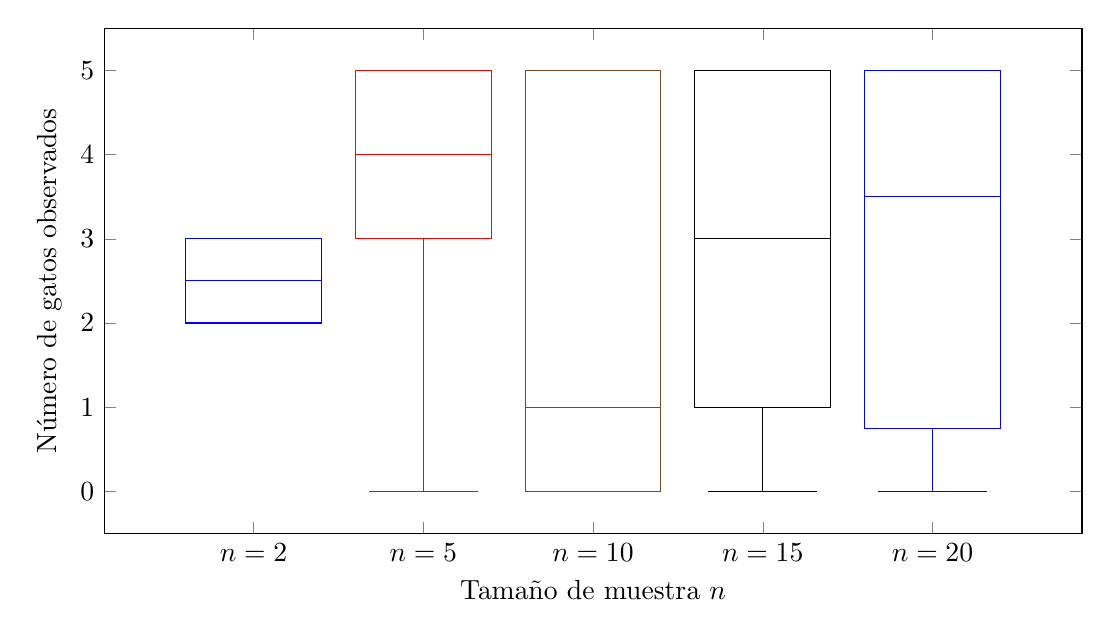
\begin{tikzpicture}
\begin{axis}[
    boxplot/draw direction=y,
    ylabel={Número de gatos observados},
    xlabel={Tamaño de muestra \(n\)},
    xtick={1,2,3,4,5},
    xticklabels={\(n=2\), \(n=5\), \(n=10\), \(n=15\), \(n=20\)},
    ymin=-0.5, ymax=5.5,
    ytick={0,1,2,3,4,5},
    width=14cm,
    height=8cm
]

\addplot+[boxplot prepared={lower whisker=2, lower quartile=2, median=2.5, upper quartile=3, upper whisker=3}] coordinates {};
\addplot+[boxplot prepared={lower whisker=0, lower quartile=3, median=4, upper quartile=5, upper whisker=5}] coordinates {};
\addplot+[boxplot prepared={lower whisker=0, lower quartile=0, median=1, upper quartile=5, upper whisker=5}] coordinates {};
\addplot+[boxplot prepared={lower whisker=0, lower quartile=1, median=3, upper quartile=5, upper whisker=5}] coordinates {};
\addplot+[boxplot prepared={lower whisker=0, lower quartile=0.75, median=3.5, upper quartile=5, upper whisker=5}] coordinates {};

\end{axis}
\end{tikzpicture}%
}
\caption{Diagramas de caja para el Equipo 1.}
\end{figure}

\subsection{El Teorema Central del Límite: aclaración fundamental}

Es común escuchar frases como:

\begin{center}
\textit{“cuando \(n\) es grande, los datos se distribuyen normal”.}
\end{center}

\textbf{Esto es incorrecto.}

El Teorema Central del Límite (TCL) no dice que la distribución de los datos originales se vuelva normal.  
Nuestros datos de gatos siguen siendo discretos (0,1,2,3,4,5) y con una forma que no es normal, incluso con \(n=20\).

\subsubsection{¿Qué dice realmente el TCL?}

El Teorema Central del Límite establece que:

\[
\boxed{\sqrt{n}\,\bigl(\bar{g} - \mu\bigr) \ \xrightarrow{d}\ \mathcal{N}(0,\sigma^2)}
\]

Es decir:

\begin{quote}
\textbf{La distribución de la media muestral \(\bar{g}\)} (no los datos individuales) se aproxima a una distribución normal conforme \(n\) aumenta.
\end{quote}

\subsubsection{Experimento mental con los gatos}

Imaginemos que repetimos muchas veces el experimento con \(n=20\):

\begin{itemize}
    \item Cada vez calculamos \(\bar{g}\) (el promedio de 20 observaciones).
    \item Esos promedios (no los gatos individuales) siguen una campana de Gauss.
\end{itemize}

Aunque un solo día veamos \(g = 0,5,2,1,3,0,5,\dots\) (discreto y no normal),  
el \textbf{promedio} de muchos días sí se comporta de manera normal.

\subsubsection{Visualización conceptual}

\begin{figure}[H]
\centering
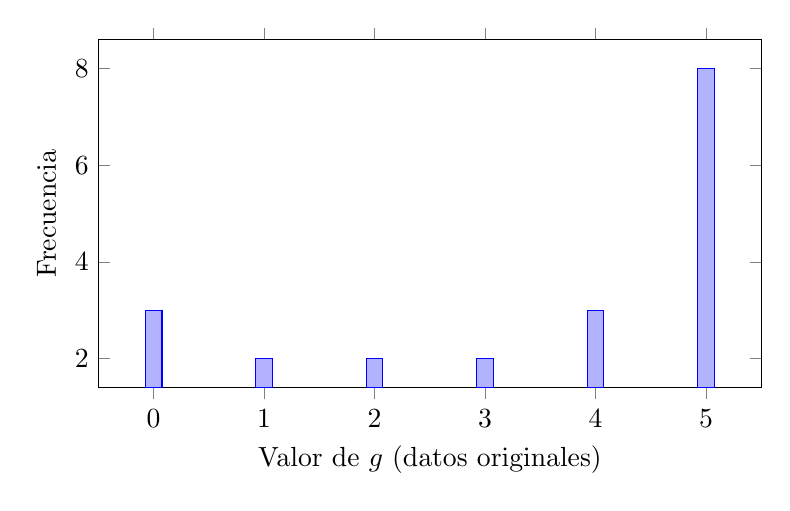
\begin{tikzpicture}
\begin{axis}[
    width=10cm,
    height=6cm,
    xlabel={Valor de \(g\) (datos originales)},
    ylabel={Frecuencia},
    ybar,
    bar width=6pt,
    xtick={0,1,2,3,4,5}
]
\addplot coordinates {(0,3) (1,2) (2,2) (3,2) (4,3) (5,8)};
\end{axis}
\end{tikzpicture}
\caption{Distribución de los datos originales (no es normal).}
\end{figure}

\begin{figure}[H]
\centering
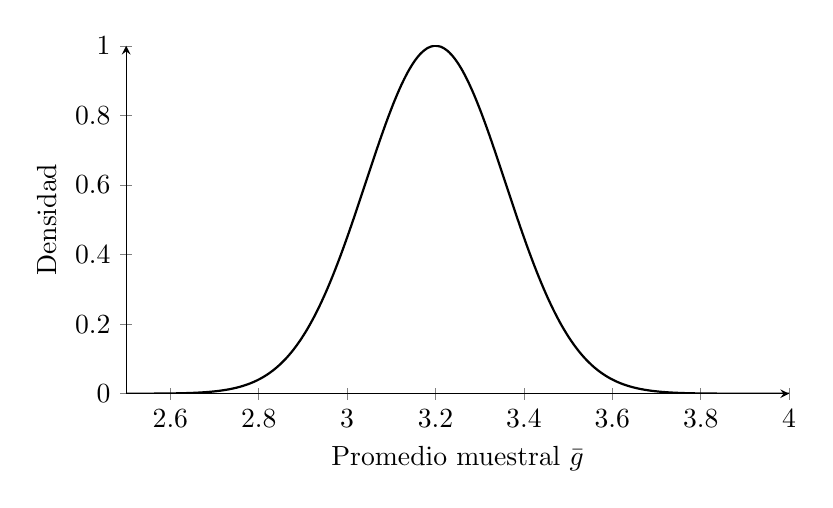
\begin{tikzpicture}
\begin{axis}[
    width=10cm,
    height=6cm,
    xlabel={Promedio muestral \(\bar{g}\)},
    ylabel={Densidad},
    domain=2.5:4.0,
    samples=100,
    axis lines=left
]
\addplot[thick, smooth] {exp(-20*(x-3.2)^2)};
\node at (axis cs:3.2,1.2) [anchor=south] {Aproximación normal};
\end{axis}
\end{tikzpicture}
\caption{Distribución de la \textbf{media muestral} \(\bar{g}\) (sí es normal).}
\end{figure}

\subsubsection{Consecuencia práctica}

\begin{quote}
\centering
\textit{El TCL nos permite usar la normal para hacer inferencias sobre la media,} \\
\textit{aunque los datos originales no sean normales.}
\end{quote}

Por eso podemos construir intervalos de confianza y pruebas de hipótesis sobre el número promedio de gatos en la UAM, incluso si cada observación individual es 0, 1, 2, 3, 4 o 5.

\subsection{Reflexión final}

Aunque el experimento parece sencillo, en realidad permite observar múltiples elementos fundamentales de estadística y probabilidad:

\begin{itemize}
\item construcción empírica de probabilidades,
\item estabilidad estadística,
\item variabilidad experimental,
\item convergencia,
\item Ley de los Grandes Números,
\item \textbf{Teorema Central del Límite}.
\end{itemize}

Más importante aún, muestra que conceptos como:

\[
\text{media},
\quad
\text{varianza},
\quad
\text{probabilidad},
\quad
\text{convergencia}
\]

no aparecen únicamente en ejercicios abstractos, sino también en fenómenos cotidianos aparentemente simples, como observar gatos dentro de una universidad.

\vspace{0.5cm}
\hrule
\vspace{0.2cm}
\begin{center}
\large
\textit{Con pocas observaciones → domina el azar} \\
\textit{Con muchas observaciones → aparece estabilidad} \\
\textit{El azar no desaparece… se organiza}
\end{center}

\begin{center}
\textbf{Eso es la Ley de los Grandes Números.}
\end{center}

\begin{center}
\textbf{Y el Teorema Central del Límite nos dice \textit{cómo} se organiza.}
\end{center}

\section[Cuando los datos desaparecen]{Cuando los datos desaparecen:\\
Limpieza, reconstrucción y análisis del comportamiento USD/MXN mediante medias móviles}

En muchos libros de estadística, ciencia de datos y aprendizaje automático, los conjuntos de datos aparecen completos y listos para analizarse. Pareciera que el investigador siempre dispone de toda la información necesaria y que los datos existen sin errores, sin huecos y sin interrupciones.

Sin embargo, en problemas reales esto rara vez ocurre. En muchas ocasiones existen fechas faltantes, errores de captura, interrupciones temporales o datos atípicos.

Esto sucede incluso en variables ampliamente monitoreadas, como el tipo de cambio USD/MXN. Aunque existen múltiples plataformas financieras, no siempre se dispone de una serie perfecta.

Por ello, antes de realizar análisis estadístico, predicción o modelado, es necesario limpiar y reconstruir los datos.

Esta práctica estudia distintas estrategias de limpieza de datos utilizando la serie histórica USD/MXN.

%===========================================================
\subsection{Fuente de datos}
%===========================================================

Fuente utilizada:

\url{https://mx.investing.com/currencies/usd-mxn-historical-data}

Periodo analizado:

\[
03/03/2025 \text{ a } 17/05/2026
\]

%===========================================================
\subsection{Objetivos del estudio}
%===========================================================

\begin{itemize}
\item Detectar fechas faltantes.
\item Detectar datos atípicos.
\item Comparar técnicas de limpieza.
\item Aplicar medias móviles de tamaño 2 a 10.
\item Comparar errores mediante MSE.
\item Analizar la distribución del error.
\end{itemize}

%===========================================================
\subsection{Variables utilizadas}
%===========================================================

\begin{table}[H]
\centering
\begin{tabular}{ll}
\toprule
Variable & Descripción\\
\midrule
Fecha & Día de observación\\
Cierre & Tipo de cambio de cierre\\
Apertura & Tipo de cambio de apertura\\
Máximo & Valor máximo diario\\
Mínimo & Valor mínimo diario\\
\% var. & Variación porcentual diaria\\
\bottomrule
\end{tabular}
\end{table}

%===========================================================
\subsection{Metodología de limpieza}
%===========================================================

%===========================================================
\subsubsection{Detección de datos faltantes}
%===========================================================

Se construye un calendario diario continuo y posteriormente se comparan las fechas observadas contra las fechas esperadas.

Esto permite identificar:

\begin{itemize}
\item fechas faltantes,
\item huecos temporales,
\item discontinuidades,
\item registros incompletos.
\end{itemize}

%===========================================================
\subsubsection{Detección de datos atípicos}
%===========================================================

Además de detectar fechas faltantes, también es importante identificar datos atípicos. Un dato atípico puede representar:

\begin{itemize}
\item un error de captura,
\item un problema de almacenamiento,
\item un cambio extraordinario del mercado,
\item o un evento financiero real.
\end{itemize}

Por ello, en esta práctica los datos atípicos se marcan para análisis, pero no se eliminan automáticamente.

%===========================================================
\paragraph{Método del rango intercuartílico (IQR)}
%===========================================================

\[
IQR = Q_3 - Q_1
\]

Un valor se considera atípico si:

\[
y_i < Q_1 - 1.5(IQR)
\]

o

\[
y_i > Q_3 + 1.5(IQR)
\]

%===========================================================
\paragraph{Método del Z-score}
%===========================================================

\[
z_i = \frac{y_i-\bar y}{s}
\]

Se considera posible dato atípico cuando:

\[
|z_i| > 3
\]

%===========================================================
\subsubsection{Técnicas de reconstrucción de datos faltantes}
%===========================================================

%===========================================================
\paragraph{Eliminación (listwise deletion)}
%===========================================================

Elimina observaciones incompletas.

\textbf{Ventajas:}
\begin{itemize}
\item no inventa información,
\item simple de implementar.
\end{itemize}

\textbf{Desventajas:}
\begin{itemize}
\item reduce tamaño de muestra,
\item rompe continuidad temporal.
\end{itemize}

%===========================================================
\paragraph{Interpolación lineal}
%===========================================================

\[
y_t =
y_{t-1}
+
\frac{y_{t+1}-y_{t-1}}{2}
\]

%===========================================================
\paragraph{Promedio local (ventana simétrica de 6 vecinos)}
%===========================================================

Se utilizan tres datos previos y tres posteriores:

\[
y_t =
\frac{
y_{t-3}+y_{t-2}+y_{t-1}
+y_{t+1}+y_{t+2}+y_{t+3}
}{6}
\]

%===========================================================
\paragraph{Promedio mensual}
%===========================================================

\[
\bar y_m =
\frac{1}{n_m}
\sum_{i=1}^{n_m} y_i
\]

%===========================================================
\subsection{Análisis mediante medias móviles}
%===========================================================

Después de limpiar los datos se aplican medias móviles:

\[
n=2,3,4,\dots,10
\]

La media móvil se define como:

\[
MM_n =
\frac{1}{n}
\sum_{i=1}^{n} y_i
\]

%===========================================================
\subsection{Métricas de evaluación}
%===========================================================

%===========================================================
\subsubsection{Error cuadrático medio (MSE)}
%===========================================================

\[
MSE =
\frac{1}{n}
\sum_{i=1}^{n}
(y_i-\hat y_i)^2
\]

donde:

\begin{itemize}
\item \(y_i\): valor observado,
\item \(\hat y_i\): valor estimado.
\end{itemize}

%===========================================================
\subsubsection{Distribución del error}
%===========================================================

El error se define como:

\[
e_i = y_i - \hat y_i
\]

Para visualizar la distribución del error se utilizan diagramas de violín.

Estos permiten observar:

\begin{itemize}
\item dispersión,
\item concentración,
\item asimetría,
\item presencia de valores extremos.
\end{itemize}

%===========================================================
\subsection{Resultados esperados}
%===========================================================

\begin{itemize}
\item Fechas faltantes detectadas.
\item Datos atípicos identificados.
\item Series reconstruidas.
\item Medias móviles calculadas.
\item Comparación de MSE entre técnicas.
\item Diagramas de violín generados.
\item Mejor técnica de limpieza identificada.
\item Mejor tamaño de ventana seleccionado.
\end{itemize}

%===========================================================
\subsection{Conclusiones}
%===========================================================

La limpieza de datos modifica directamente los resultados del análisis. En series financieras, la manera en que se reconstruyen datos faltantes puede alterar tendencias, errores y conclusiones.

Por ello, antes de aplicar modelos estadísticos o predictivos, es necesario comprender qué técnica de limpieza se utiliza y cómo afecta los resultados.

%===========================================================
%===========================================================

%===========================================================
\subsection{Anexo A: Pseudocódigo del procedimiento}
%===========================================================

\begin{verbatim}
INICIO

Leer datos USD/MXN

Construir calendario completo

Detectar:
    Fechas faltantes
    Datos atípicos

Aplicar técnicas de reconstruccion:
    Eliminacion
    Interpolacion lineal
    Promedio local
    Promedio mensual

Calcular:
    Medias moviles (n = 2 a 10)
    MSE para cada media movil
    Distribucion del error

Comparar resultados entre tecnicas

FIN
\end{verbatim}

%===========================================================
\subsection{Anexo B: Muestra de datos utilizados}
%===========================================================

\begin{verbatim}
15/05/2026 17.3400 17.2215 17.4085 17.2090 +0.69%
14/05/2026 17.2215 17.1775 17.2490 17.1575 +0.26%
13/05/2026 17.1775 17.2280 17.2582 17.1629 -0.27%
12/05/2026 17.2239 17.2025 17.2850 17.1805 +0.15%
11/05/2026 17.1975 17.1915 17.2391 17.1587 -0.11%
10/05/2026 17.2171 17.1810 17.2525 17.2090 +0.20%
...
03/03/2025 20.6860 20.5265 20.7505 20.3722 +0.75%
\end{verbatim}

%===========================================================
\subsection{Anexo C: Implementación en Python}
%===========================================================

\begin{lstlisting}[language=Python]
import pandas as pd
import numpy as np
import matplotlib.pyplot as plt
import re

raw_text = """
PEGAR AQUI LOS DATOS COMPLETOS
"""

patron = re.compile(
    r"(\d{2}/\d{2}/\d{4})\s+"
    r"([\d.]+)\s+"
    r"([\d.]+)\s+"
    r"([\d.]+)\s+"
    r"([\d.]+)\s+"
    r"([+-]?[\d.]+)%"
)

filas = []

for linea in raw_text.splitlines():

    m = patron.search(linea)

    if m:
        filas.append(m.groups())

df = pd.DataFrame(
    filas,
    columns=[
        "Fecha",
        "Cierre",
        "Apertura",
        "Maximo",
        "Minimo",
        "Var_pct"
    ]
)

df["Fecha"] = pd.to_datetime(
    df["Fecha"],
    format="%d/%m/%Y"
)

for col in [
    "Cierre",
    "Apertura",
    "Maximo",
    "Minimo",
    "Var_pct"
]:
    df[col] = pd.to_numeric(
        df[col],
        errors="coerce"
    )

# DETECCION DE ATIPICOS CON IQR

def detectar_atipicos_iqr(data, columna):

    q1 = data[columna].quantile(0.25)
    q3 = data[columna].quantile(0.75)

    iqr = q3 - q1

    li = q1 - 1.5 * iqr
    ls = q3 + 1.5 * iqr

    return (
        (data[columna] < li) |
        (data[columna] > ls)
    )

df["Atipico"] = detectar_atipicos_iqr(
    df,
    "Cierre"
)

# CREACION DE CALENDARIO COMPLETO

calendario = pd.DataFrame({
    "Fecha": pd.date_range(
        df["Fecha"].min(),
        df["Fecha"].max(),
        freq="D"
    )
})

df_completo = calendario.merge(
    df,
    on="Fecha",
    how="left"
)

# INTERPOLACION LINEAL

columnas_numericas = [
    "Cierre",
    "Apertura",
    "Maximo",
    "Minimo",
    "Var_pct"
]

df_interpolacion = df_completo.copy()

df_interpolacion[columnas_numericas] = (
    df_interpolacion[columnas_numericas]
    .interpolate(method="linear")
)

# CALCULO DE MEDIAS MOVILES

for n in range(2,11):

    df_interpolacion[f"MM_{n}"] = (
        df_interpolacion["Cierre"]
        .rolling(window=n, min_periods=1)
        .mean()
    )

# FUNCION PARA CALCULAR MSE

def calcular_mse(real, predicho):

    return np.mean(
        (real - predicho)**2
    )

# TABLA DE ERRORES POR VENTANA

tabla_errores = []

for n in range(2,11):

    mse = calcular_mse(
        df_interpolacion["Cierre"],
        df_interpolacion[f"MM_{n}"]
    )

    tabla_errores.append({
        "n": n,
        "MSE": mse
    })

tabla_errores = pd.DataFrame(
    tabla_errores
)

print(tabla_errores)

# DIAGRAMA DE VIOLIN DE ERRORES

errores = []

for n in range(2,11):

    temp = (
        df_interpolacion["Cierre"]
        -
        df_interpolacion[f"MM_{n}"]
    )

    errores.append(
        temp.dropna()
    )

plt.figure(figsize=(12,6))

plt.violinplot(
    errores,
    showmeans=True,
    showmedians=True
)

plt.xticks(
    range(1,10),
    [f"MM_{n}" for n in range(2,11)]
)

plt.title(
    "Distribucion del error por media movil"
)

plt.grid(True)

plt.show()
\end{lstlisting}

\section{Experimento: ¿Miel, azúcar o café?}

\subsection{Introducción}

En distintos sistemas de cultivo artesanal y huertos caseros suele mencionarse que algunas sustancias comunes pueden favorecer el crecimiento vegetal. Entre las más utilizadas aparecen la miel, el azúcar y el café soluble.

Frecuentemente se escuchan comentarios como:

\begin{quote}
“La miel contiene nutrientes y podría favorecer el crecimiento.”
\end{quote}

o bien:

\begin{quote}
“El café ayuda a estimular las plantas.”
\end{quote}

Sin embargo, muchas de estas afirmaciones provienen únicamente de observaciones empíricas y no de experimentos controlados.

Por esta razón se desarrolló un experimento utilizando semillas de lenteja con el objetivo de evaluar si distintos tratamientos generan diferencias observables en la germinación y desarrollo inicial de las plantas.

Además de estudiar el crecimiento vegetal, esta práctica permite introducir conceptos fundamentales del Diseño y Análisis de Experimentos, tales como:

\begin{itemize}
    \item unidad experimental,
    \item factor,
    \item niveles,
    \item réplicas,
    \item variabilidad experimental,
    \item análisis de medias,
    \item y ANOVA.
\end{itemize}

\subsection{Pregunta de investigación}

\begin{center}
\textit{¿Existen diferencias en la germinación y crecimiento de lentejas al aplicar miel, azúcar o café soluble?}
\end{center}

\subsection{Hipótesis}

\subsubsection{Hipótesis nula}

\[
H_0:\mu_B=\mu_M=\mu_A=\mu_C
\]

No existen diferencias significativas entre las medias de los tratamientos.

\subsubsection{Hipótesis alternativa}

\[
H_1:\text{Al menos una media es diferente}
\]

\subsection{Objetivo general}

Evaluar el efecto de distintos tratamientos sobre la germinación y crecimiento inicial de semillas de lenteja mediante un diseño experimental completamente aleatorizado y análisis ANOVA.

\section{Materiales y métodos}

\subsection{Materiales}

\begin{itemize}
    \item Agua
    \item Grenetina
    \item Azúcar
    \item Café soluble
    \item Miel
    \item Agua oxigenada comercial
    \item Antihongos comercial
    \item Semillas de lenteja
    \item Pipetas
    \item Báscula
    \item Recipientes plásticos transparentes
    \item Regla milimétrica
\end{itemize}

\subsection{Construcción del medio semisólido}

Para construir el medio de cultivo se utilizaron las siguientes cantidades:

\begin{table}[H]
\centering
\begin{tabular}{lc}
\toprule
Componente & Cantidad \\
\midrule
Agua & 2000 g \\
Grenetina & 100 g \\
Azúcar & 100 g \\
Agua oxigenada & 30 g \\
Antihongos & 0.5 g \\
\bottomrule
\end{tabular}
\caption{Composición del medio base}
\end{table}

\subsection{Preparación del medio}

\begin{enumerate}
    \item Calentar el agua.
    \item Agregar grenetina y azúcar.
    \item Llevar a ebullición.
    \item Mantener el hervor durante cinco minutos.
    \item Retirar del fuego.
    \item Esperar ligera disminución de temperatura.
    \item Agregar agua oxigenada y antihongos.
    \item Mezclar cuidadosamente.
    \item Colocar aproximadamente 30 g de medio por recipiente.
\end{enumerate}

\section{Tratamientos experimentales}

Cada solución fue preparada utilizando:

\[
30\text{ g de agua} + 30\text{ g de soluto}
\]

\begin{table}[H]
\centering
\begin{tabular}{ccc}
\toprule
Color & Tratamiento & Código \\
\midrule
Amarillo & Blanco & B \\
Morado & Miel & M \\
Azul & Azúcar & A \\
Verde & Café soluble & C \\
\bottomrule
\end{tabular}
\caption{Tratamientos experimentales}
\end{table}

\subsection{Aplicación experimental}

\begin{itemize}
    \item Se utilizaron 6 semillas por recipiente.
    \item Cada tratamiento fue realizado por triplicado.
    \item Las semillas fueron previamente hidratadas.
    \item Se aplicaron 3 gotas del tratamiento correspondiente.
    \item Los recipientes permanecieron cerrados.
    \item Las observaciones fueron realizadas diariamente.
\end{itemize}

\section{Diseño experimental}

\begin{itemize}
    \item Factor: tratamiento aplicado
    \item Niveles: 4
    \item Réplicas: 3
    \item Diseño: completamente aleatorizado
\end{itemize}

El número total de unidades experimentales fue:

\[
4\times3=12
\]

\subsection{Unidad experimental}

La unidad experimental corresponde al recipiente y no a cada semilla individual.

Esto es importante porque todas las semillas dentro de un mismo recipiente comparten:

\begin{itemize}
    \item humedad,
    \item temperatura,
    \item iluminación,
    \item y concentración del tratamiento.
\end{itemize}

\section{Variables evaluadas}

Durante el experimento se registraron:

\begin{itemize}
    \item Número de semillas germinadas
    \item Longitud de raíz
    \item Altura del tallo
    \item Presencia de hojas
    \item Presencia de hongos
    \item Condensación
\end{itemize}

\section{Estrategia temporal de análisis}

Aunque el experimento fue monitoreado diariamente, únicamente se reportarán medias correspondientes a:

\begin{itemize}
    \item Día 2
    \item Día 4
    \item Día 20
\end{itemize}

Estos tiempos representan distintas etapas del desarrollo experimental:

\begin{itemize}
    \item Día 2: germinación inicial,
    \item Día 4: establecimiento temprano,
    \item Día 20: desarrollo consolidado.
\end{itemize}

El análisis estadístico inferencial mediante ANOVA fue realizado exclusivamente utilizando los datos correspondientes al día 20, debido a que este punto temporal representa el estado final del sistema experimental bajo condiciones homogéneas de exposición.

\section{Tabla general de registro}

\begin{table}[H]
\centering
\resizebox{\linewidth}{!}{
\begin{tabular}{lcccccc}
\toprule
Tratamiento & Réplica & Día 2 & Día 4 & Día 20 & Hongos & Observaciones \\
\midrule
Blanco & 1 & & & & & \\
Blanco & 2 & & & & & \\
Blanco & 3 & & & & & \\
\midrule
Miel & 1 & & & & & \\
Miel & 2 & & & & & \\
Miel & 3 & & & & & \\
\midrule
Azúcar & 1 & & & & & \\
Azúcar & 2 & & & & & \\
Azúcar & 3 & & & & & \\
\midrule
Café & 1 & & & & & \\
Café & 2 & & & & & \\
Café & 3 & & & & & \\
\bottomrule
\end{tabular}
}
\caption{Registro experimental resumido}
\end{table}

\section{Cálculo de medias experimentales}

A partir de las mediciones registradas en las fotografías correspondientes al día 20 del experimento, se calcularon las medias de crecimiento para cada tratamiento.

En el tratamiento con miel se registraron las siguientes longitudes de raíz:

\[
4.2,\ 4.5,\ 5.1 \text{ cm}
\]

La media experimental fue calculada mediante:

\[
\bar{x}=\frac{\sum_{i=1}^{n}x_i}{n}
\]

Sustituyendo los valores experimentales:

\[
\bar{x}=\frac{4.2+4.5+5.1}{3}
\]

\[
\bar{x}=\frac{13.8}{3}
\]

\[
\bar{x}=4.6\text{ cm}
\]

\section{Cálculo de varianza}

La dispersión experimental fue estimada mediante la varianza muestral:

\[
s^2=\frac{\sum_{i=1}^{n}(x_i-\bar{x})^2}{n-1}
\]

Sustituyendo los valores observados:

\[
s^2=\frac{
(4.2-4.6)^2+
(4.5-4.6)^2+
(5.1-4.6)^2
}{2}
\]

\[
s^2=
\frac{
0.16+0.01+0.25
}{2}
\]

\[
s^2=
\frac{0.42}{2}
\]

\[
s^2=0.21
\]

\section{Análisis ANOVA}

El análisis ANOVA permite determinar si las diferencias observadas entre tratamientos son suficientemente grandes como para pensar que existe un efecto real asociado al tratamiento aplicado.

\subsection{Estadístico F}

\[
F=\frac{CM_{Tratamientos}}{CM_{Error}}
\]

donde:

\begin{itemize}
    \item $CM_{Tratamientos}$ corresponde al cuadrado medio entre tratamientos,
    \item $CM_{Error}$ corresponde al cuadrado medio del error experimental.
\end{itemize}

Si:

\[
p<0.05
\]

entonces se rechaza la hipótesis nula.

\section{Tabla ANOVA}

\begin{table}[H]
\centering
\begin{tabular}{lcccc}
\toprule
Fuente & SC & gl & CM & F \\
\midrule
Tratamientos & & & & \\
Error & & & & \\
Total & & & & \\
\bottomrule
\end{tabular}
\caption{Tabla ANOVA}
\end{table}

\section{Interpretación biológica}

Si el ANOVA no presenta diferencias significativas, entonces las variaciones observadas entre tratamientos podrían atribuirse al azar experimental.

Por el contrario, si el análisis presenta diferencias significativas, entonces al menos uno de los tratamientos estaría afectando el crecimiento vegetal de manera distinta.

En ese caso podrían realizarse pruebas post-hoc, como Tukey, para identificar específicamente qué tratamientos difieren entre sí.

\section{Conclusiones}

El experimento permitió integrar observación biológica, medición experimental y análisis estadístico dentro de un mismo sistema de estudio.

La utilización de tratamientos como miel, azúcar y café soluble permitió construir un escenario experimental adecuado para introducir conceptos fundamentales del Diseño y Análisis de Experimentos.

El uso de réplicas permitió estimar variabilidad experimental, mientras que el análisis ANOVA proporcionó una herramienta formal para comparar tratamientos bajo condiciones homogéneas.

La decisión de utilizar únicamente las mediciones correspondientes al día 20 para el análisis inferencial permitió homogenizar temporalmente las comparaciones y reducir problemas asociados a mediciones repetidas dependientes.

Finalmente, el experimento muestra cómo observaciones aparentemente simples pueden transformarse en un análisis científico estructurado mediante:

\begin{itemize}
    \item control experimental,
    \item medición,
    \item estadística,
    \item y análisis cuantitativo.
\end{itemize}
\section{\texorpdfstring{Sustancias, interacciones y cambios visuales en papel: introducción al diseño factorial \(2^2\)}{Sustancias, interacciones y cambios visuales en papel: introducción al diseño factorial 2 por 2}}

\subsection{Introducción}

Las organizaciones frecuentemente deben tomar decisiones acerca de qué materiales, procesos o tratamientos producen mejores resultados. Sin embargo, cuando intervienen varios factores simultáneamente, resulta difícil determinar cuál de ellos es responsable de los cambios observados.

Una estrategia ampliamente utilizada para abordar este problema consiste en emplear diseños experimentales factoriales. Estos diseños permiten estudiar simultáneamente varios factores, evaluar sus efectos individuales y analizar posibles interacciones entre ellos.

En esta práctica se utilizarán soluciones elaboradas con cúrcuma y cloro comercial aplicadas sobre papel adhesivo (\textit{post-it}) para generar cambios visuales observables. Aunque el sistema experimental es sencillo, reproduce la lógica utilizada en numerosos experimentos industriales, agrícolas y científicos.

El objetivo principal no consiste en estudiar las propiedades químicas de la cúrcuma o del cloro, sino comprender cómo se construye un diseño factorial, cómo se establecen tratamientos experimentales, cuál es la función de un blanco experimental y cómo se registran e interpretan los resultados obtenidos.

Además, se incorporará el uso de un luxómetro para transformar observaciones visuales en mediciones cuantitativas, permitiendo analizar los tratamientos mediante herramientas estadísticas objetivas.

\subsection{Objetivo general}

Comprender la estructura y aplicación de un diseño factorial $2^2$ mediante el análisis de cambios visuales y de transmisión luminosa producidos por soluciones de cúrcuma y cloro comercial sobre papel.

\subsection{Objetivos particulares}

\begin{itemize}
\item Identificar factores, niveles y tratamientos experimentales.
\item Comprender la función de un blanco experimental.
\item Analizar la importancia de las repeticiones experimentales.
\item Registrar y comparar cambios visuales producidos por diferentes tratamientos.
\item Introducir el concepto de interacción entre factores.
\item Medir cuantitativamente la transmisión luminosa utilizando un luxómetro.
\item Generar evidencia experimental para la toma de decisiones.
\end{itemize}

\subsection{Fundamento teórico}

Los diseños factoriales permiten estudiar simultáneamente el efecto de varios factores sobre una o más variables respuesta. Cuando se analizan dos factores y cada uno posee dos niveles, se obtiene un diseño factorial:

\[
2^2
\]

Este diseño genera cuatro combinaciones experimentales diferentes y permite estimar:

\begin{itemize}
\item el efecto principal del primer factor,
\item el efecto principal del segundo factor,
\item y la posible interacción entre ambos factores.
\end{itemize}

La principal ventaja de este enfoque es que permite obtener más información utilizando un número relativamente pequeño de tratamientos experimentales.

\subsection{Contexto del problema}

Una empresa dedicada a la fabricación de materiales decorativos desea desarrollar papeles con distintos efectos visuales. Antes de invertir en producción necesita determinar qué combinación de sustancias genera los cambios más interesantes y qué tratamientos modifican la transmisión de luz a través del papel.

Para responder estas preguntas se diseñará un experimento controlado utilizando cúrcuma y cloro comercial como factores experimentales.

\subsection{Factores experimentales}

En esta práctica se estudiarán dos factores.

\subsubsection{Factor A: concentración de cúrcuma}

\begin{table}[H]
\centering
\begin{tabular}{cc}
\hline
Nivel & Concentración \\
\hline
Bajo (-) & 1 g \\
Alto (+) & 4 g \\
\hline
\end{tabular}
\caption{Niveles del factor cúrcuma.}
\end{table}

\subsubsection{Factor B: concentración de cloro comercial}

\begin{table}[H]
\centering
\begin{tabular}{cc}
\hline
Nivel & Concentración \\
\hline
Bajo (-) & 5 g \\
Alto (+) & 10 g \\
\hline
\end{tabular}
\caption{Niveles del factor cloro comercial.}
\end{table}

\subsection{Variables controladas}

Con el propósito de que los cambios observados puedan atribuirse a los factores estudiados, todos los tratamientos mantendrán constantes las siguientes condiciones:

\begin{itemize}
\item 350 g de agua potable.
\item 20 g de sal.
\item Tres aspersiones por unidad experimental.
\item Distancia de aplicación de 10 cm.
\item Mismo tipo de papel adhesivo.
\item Mismo tiempo de secado.
\item Mismo tamaño de la pieza de madera utilizada para cubrir parcialmente el papel.
\end{itemize}

\subsection{Diseño experimental}

La estructura factorial utilizada se muestra en la Tabla \ref{tab:factorial}.

\begin{table}[H]
\centering
\caption{Tratamientos factoriales del diseño $2^2$.}
\label{tab:factorial}
\begin{tabular}{ccc}
\hline
Tratamiento & Cúrcuma & Cloro \\
\hline
T1 & 1 g & 5 g \\
T2 & 1 g & 10 g \\
T3 & 4 g & 5 g \\
T4 & 4 g & 10 g \\
\hline
\end{tabular}
\end{table}

\subsection{Blanco experimental}

Además de los tratamientos factoriales se incorporará un blanco experimental compuesto únicamente por:

\[
350 \text{ g de agua potable}
\]

y

\[
20 \text{ g de sal}
\]

sin cúrcuma y sin cloro comercial.

La función del blanco es proporcionar una referencia para determinar si los cambios observados son consecuencia de los factores estudiados o simplemente resultado de la humedad o del proceso de aplicación.

\subsection{Unidad experimental}

La unidad experimental corresponderá a un post-it individual.

Cada tratamiento contará con seis repeticiones independientes.

Por lo tanto, el número total de unidades experimentales será:

\[
5 \times 6 = 30
\]

donde los cinco tratamientos corresponden a los cuatro tratamientos factoriales y al blanco experimental.

\subsection{Preparación de las soluciones}

Las soluciones se prepararán al menos 24 horas antes de la aplicación experimental.

El objetivo de este periodo de reposo es permitir una adecuada dispersión de los componentes y garantizar condiciones homogéneas entre tratamientos.

Cada solución contendrá:

\begin{itemize}
\item 350 g de agua potable,
\item 20 g de sal,
\item y las cantidades correspondientes de cúrcuma y cloro según el tratamiento asignado.
\end{itemize}

\begin{table}[H]
\centering
\begin{tabular}{cccc}
\hline
Tratamiento & Cúrcuma & Cloro & Sal \\
\hline
T1 & 1 g & 5 g & 20 g \\
T2 & 1 g & 10 g & 20 g \\
T3 & 4 g & 5 g & 20 g \\
T4 & 4 g & 10 g & 20 g \\
B1 & 0 g & 0 g & 20 g \\
\hline
\end{tabular}
\caption{Composición de los tratamientos experimentales.}
\end{table}

\subsection{Procedimiento experimental}

\begin{enumerate}
\item Colocar un post-it sobre una superficie plana.

\item Cubrir aproximadamente la mitad de la superficie mediante una pieza de madera.

\item Colocar el atomizador inclinado respecto al papel.

\item Mantener una distancia aproximada de:

\[
10 \text{ cm}
\]

entre el atomizador y la superficie experimental.

\item Aplicar tres aspersiones sobre la muestra.

\item Retirar cuidadosamente la pieza de madera.

\item Dejar secar la muestra bajo las mismas condiciones ambientales.

\item Registrar fotografías y observaciones.
\end{enumerate}

\subsection{Variables respuesta}

La práctica considera variables tanto cualitativas como cuantitativas.

\subsubsection{Variables cualitativas}

\begin{itemize}
\item Intensidad visual del color.
\item Uniformidad de la coloración.
\item Contraste entre zonas protegidas y expuestas.
\item Atractivo visual.
\end{itemize}

\subsubsection{Variables cuantitativas}

La variable principal será la transmisión luminosa medida mediante un luxómetro.

\[
L=\text{lux medidos}
\]

Esta variable permitirá cuantificar la cantidad de luz que atraviesa cada unidad experimental.

\subsection{Medición mediante luxómetro}

Una vez que las muestras hayan secado completamente, se procederá a medir la transmisión luminosa utilizando un luxómetro.

Para ello se utilizará una fuente de luz constante colocada debajo de la muestra.

El montaje experimental será:

\[
\text{Fuente de luz} \rightarrow \text{Post-it} \rightarrow \text{Luxómetro}
\]

Primero se registrará la intensidad luminosa sin muestra:

\[
L_0
\]

Posteriormente se registrará la intensidad luminosa atravesando cada post-it tratado:

\[
L_i
\]

Con estos valores podrá calcularse el porcentaje de bloqueo de luz:

\[
\%B=
\frac{L_0-L_i}{L_0}\times100
\]

donde:

\begin{itemize}
\item $L_0$ corresponde a la lectura sin muestra.
\item $L_i$ corresponde a la lectura con la muestra.
\end{itemize}

\subsection{Tabla de registro experimental}

\begin{table}[H]
\centering
\resizebox{0.98\linewidth}{!}{%
\begin{tabular}{ccccccccc}
\hline
Trat. & Rep. & Lux & \% Bloqueo & Color & Contraste & Uniformidad & Atractivo & Obs. \\
\hline
T1 & 1 & & & & & & & \\
T1 & 2 & & & & & & & \\
T1 & 3 & & & & & & & \\
T1 & 4 & & & & & & & \\
T1 & 5 & & & & & & & \\
T1 & 6 & & & & & & & \\
\hline
\end{tabular}%
}
\caption{Formato de captura de datos experimentales.}
\end{table}

\subsection{Análisis de resultados}

Con los datos obtenidos se podrá:

\begin{itemize}
\item Calcular promedios por tratamiento.
\item Comparar tratamientos utilizando diagramas de caja.
\item Construir gráficas de efectos principales.
\item Analizar posibles interacciones entre factores.
\item Realizar un ANOVA factorial utilizando la variable lux como respuesta principal.
\end{itemize}

\subsubsection{\texorpdfstring{Análisis estadístico mediante ANOVA factorial \(2^2\)}{Análisis estadístico mediante ANOVA factorial 2 por 2}}

Para analizar cuantitativamente los resultados se utiliza un modelo estadístico lineal que permite descomponer la variabilidad total observada en componentes atribuibles a cada factor y a su interacción.

\paragraph{Modelo estadístico}

\[
Y_{ijk} = \mu + A_i + B_j + (AB)_{ij} + \varepsilon_{ijk}
\]

donde:
\begin{itemize}
\item $Y_{ijk}$: variable respuesta (porcentaje de bloqueo de luz) para la réplica $k$ en la combinación de niveles $i$ de cúrcuma y $j$ de cloro.
\item $\mu$: media global del experimento.
\item $A_i$: efecto del factor cúrcuma en el nivel $i$ (bajo o alto).
\item $B_j$: efecto del factor cloro en el nivel $j$ (bajo o alto).
\item $(AB)_{ij}$: efecto de interacción entre cúrcuma y cloro.
\item $\varepsilon_{ijk}$: error experimental, que se asume aleatorio, independiente y distribuido normalmente con media cero y varianza constante.
\end{itemize}

\paragraph{Codificación de niveles y tratamientos}

Para facilitar los cálculos, se asigna el valor $-$ al nivel bajo y $+$ al nivel alto de cada factor.

\begin{table}[H]
\centering
\resizebox{0.98\linewidth}{!}{%
\begin{tabular}{ccccc}
\hline
Tratamiento & Cúrcuma (A) & Cloro (B) & Codificación & Promedio \% bloqueo \\
\hline
T1 & 1 g ($-$) & 5 g ($-$) & $(-,-)$ & $\overline{Y}_1$ \\
T2 & 1 g ($-$) & 10 g (+) & $(-,+)$ & $\overline{Y}_2$ \\
T3 & 4 g (+) & 5 g ($-$) & $(+,-)$ & $\overline{Y}_3$ \\
T4 & 4 g (+) & 10 g (+) & $(+,+)$ & $\overline{Y}_4$ \\
\hline
\end{tabular}%
}
\caption{Codificación de niveles y promedios por tratamiento.}
\end{table}

\paragraph{Cálculo de efectos principales e interacción}

Los efectos se estiman mediante contrastes ortogonales utilizando los signos $+$ y $-$.

\textbf{Efecto principal de A (cúrcuma):}

Compara el promedio de los tratamientos con nivel alto de cúrcuma contra los de nivel bajo.

\[
\text{Efecto}_A = \frac{(\overline{Y}_3 + \overline{Y}_4)}{2} - \frac{(\overline{Y}_1 + \overline{Y}_2)}{2}
\]

En forma de contraste con signos:

\[
\text{Efecto}_A = \frac{-\overline{Y}_1 - \overline{Y}_2 + \overline{Y}_3 + \overline{Y}_4}{2}
\]

\textbf{Efecto principal de B (cloro):}

Compara el promedio de los tratamientos con nivel alto de cloro contra los de nivel bajo.

\[
\text{Efecto}_B = \frac{(\overline{Y}_2 + \overline{Y}_4)}{2} - \frac{(\overline{Y}_1 + \overline{Y}_3)}{2}
\]

En forma de contraste con signos:

\[
\text{Efecto}_B = \frac{-\overline{Y}_1 + \overline{Y}_2 - \overline{Y}_3 + \overline{Y}_4}{2}
\]

\textbf{Interacción AB:}

Mide si el efecto de un factor depende del nivel del otro factor.

\[
\text{Efecto}_{AB} = \frac{(\overline{Y}_1 + \overline{Y}_4)}{2} - \frac{(\overline{Y}_2 + \overline{Y}_3)}{2}
\]

En forma de contraste con signos:

\[
\text{Efecto}_{AB} = \frac{+\overline{Y}_1 - \overline{Y}_2 - \overline{Y}_3 + \overline{Y}_4}{2}
\]

\paragraph{Sumas de cuadrados (SC)}

Cada contraste se construye con las sumas de las repeticiones, no con los promedios. Sea $n$ el número de repeticiones por tratamiento (en este caso $n=6$).

\textbf{Contraste para A:}

\[
\text{Contraste}_A = -\sum_{k=1}^{n} Y_{1k} -\sum_{k=1}^{n} Y_{2k} +\sum_{k=1}^{n} Y_{3k} +\sum_{k=1}^{n} Y_{4k}
\]

\textbf{Suma de cuadrados para A:}

\[
SC_A = \frac{(\text{Contraste}_A)^2}{4n}
\]

\textbf{Análogamente para B y AB:}

\[
SC_B = \frac{(\text{Contraste}_B)^2}{4n}, \quad SC_{AB} = \frac{(\text{Contraste}_{AB})^2}{4n}
\]

\textbf{Suma de cuadrados total:}

\[
SC_{\text{total}} = \sum_{i=1}^{4} \sum_{k=1}^{n} Y_{ik}^2 - \frac{(\sum_{i=1}^{4} \sum_{k=1}^{n} Y_{ik})^2}{4n}
\]

\textbf{Suma de cuadrados del error:}

\[
SC_{\text{error}} = SC_{\text{total}} - (SC_A + SC_B + SC_{AB})
\]

\paragraph{Cuadrados medios (CM) y estadístico F}

Los cuadrados medios se obtienen dividiendo cada suma de cuadrados entre sus grados de libertad (gl):

\begin{itemize}
\item Factor A: gl = 1
\item Factor B: gl = 1
\item Interacción AB: gl = 1
\item Error: gl = $4(n-1) = 4(6-1) = 20$
\item Total: gl = $4n - 1 = 23$
\end{itemize}

\[
CM_A = \frac{SC_A}{1}, \quad CM_B = \frac{SC_B}{1}, \quad CM_{AB} = \frac{SC_{AB}}{1}, \quad CM_{\text{error}} = \frac{SC_{\text{error}}}{4(n-1)}
\]

El estadístico $F$ para cada fuente se calcula como:

\[
F_A = \frac{CM_A}{CM_{\text{error}}}, \quad F_B = \frac{CM_B}{CM_{\text{error}}}, \quad F_{AB} = \frac{CM_{AB}}{CM_{\text{error}}}
\]

Cada $F$ se compara con el valor crítico de la distribución $F$ con 1 y $4(n-1)$ grados de libertad para determinar si el efecto es estadísticamente significativo.

\paragraph{Tabla de ANOVA}

\begin{table}[H]
\centering
\begin{tabular}{lccccc}
\hline
Fuente de variación & SC & gl & CM & F & p-valor \\
\hline
Cúrcuma (A) & $SC_A$ & 1 & $CM_A$ & $F_A$ & \\
Cloro (B) & $SC_B$ & 1 & $CM_B$ & $F_B$ & \\
Interacción AB & $SC_{AB}$ & 1 & $CM_{AB}$ & $F_{AB}$ & \\
Error & $SC_{\text{error}}$ & $4(n-1)$ & $CM_{\text{error}}$ & & \\
\hline
Total & $SC_{\text{total}}$ & $4n-1$ & & & \\
\hline
\end{tabular}
\caption{Tabla de ANOVA para el diseño factorial $2^2$.}
\end{table}

\paragraph{Interpretación de resultados}

\begin{itemize}
\item Si $F_A$ es mayor que el valor crítico (o el p-valor < 0.05), se concluye que la concentración de cúrcuma afecta significativamente el bloqueo de luz.
\item Si $F_B$ es significativo, el cloro tiene un efecto significativo.
\item Si $F_{AB}$ es significativo, existe interacción: el efecto de un factor depende del nivel del otro.
\end{itemize}

La ventaja de este análisis es que transforma observaciones visuales subjetivas en decisiones objetivas basadas en evidencia estadística.

\subsubsection{Ejemplo ilustrativo (datos hipotéticos)}

Supóngase que con $n=6$ repeticiones se obtienen los siguientes promedios de porcentaje de bloqueo de luz:

\begin{itemize}
\item T1 ($-$,$-$): 10\%
\item T2 ($-$,$+$): 25\%
\item T3 ($+$,$-$): 30\%
\item T4 ($+$,$+$): 60\%
\end{itemize}

Aplicando las fórmulas:

\[
\text{Efecto}_A = \frac{30+60}{2} - \frac{10+25}{2} = 45 - 17.5 = 27.5\%
\]

\[
\text{Efecto}_B = \frac{25+60}{2} - \frac{10+30}{2} = 42.5 - 20 = 22.5\%
\]

\[
\text{Efecto}_{AB} = \frac{10+60}{2} - \frac{25+30}{2} = 35 - 27.5 = 7.5\%
\]

Interpretación:
\begin{itemize}
\item Pasar de 1 g a 4 g de cúrcuma aumenta el bloqueo en 27.5\%.
\item Pasar de 5 g a 10 g de cloro aumenta el bloqueo en 22.5\%.
\item La interacción positiva (7.5\%) indica que el efecto combinado de ambos factores es ligeramente mayor que la suma de sus efectos individuales.
\end{itemize}

Con un ANOVA se determinaría si estos efectos son estadísticamente significativos.

\subsection{Preguntas de análisis}

\begin{enumerate}
\item ¿Qué diferencia existe entre un factor y un nivel?
\item ¿Por qué este experimento corresponde a un diseño factorial $2^2$?
\item ¿Qué función cumple el blanco experimental?
\item ¿Por qué se utilizan repeticiones?
\item ¿Qué tratamiento produjo el mayor cambio visual?
\item ¿Qué tratamiento produjo el mayor bloqueo de luz?
\item ¿Existe evidencia de interacción entre la cúrcuma y el cloro?
\item ¿Qué ocurriría si se eliminara el blanco experimental?
\item ¿Qué ventaja tiene utilizar un luxómetro en lugar de únicamente observaciones visuales?
\item ¿Qué variable utilizarías para realizar un ANOVA y por qué?
\end{enumerate}

\subsection{Reflexión final}

Aunque el sistema experimental utiliza materiales sencillos, reproduce los principios fundamentales empleados en investigación científica y desarrollo tecnológico. Comprender cómo se diseñan los tratamientos, cómo se controlan las variables y cómo se interpretan los resultados constituye una habilidad esencial para la toma de decisiones basada en evidencia.

La incorporación del luxómetro permite además distinguir entre observaciones subjetivas y mediciones instrumentales, fortaleciendo la calidad de las conclusiones obtenidas. El uso del ANOVA factorial con la variable cuantitativa de porcentaje de bloqueo de luz permite decidir estadísticamente si los efectos observados son reales o debidos al azar, tal como se hace en la industria farmacéutica, agrícola y de manufactura para optimizar procesos.
\section{Más allá de los factores: diseño Taguchi para analizar hojas de violeta africana en sistemas biológicos confinados}

\subsection{Introducción}

A muchas personas les gustan las plantas y desearían reproducirlas para tener más ejemplares en casa, en un laboratorio o en un espacio de aprendizaje. Entre las plantas ornamentales más interesantes para este propósito se encuentran las violetas africanas, ya que pueden reproducirse vegetativamente a partir de sus hojas.

Sin embargo, la propagación vegetal no siempre ocurre con éxito. Si la hoja pierde humedad, se contamina, se corta de forma inadecuada o no encuentra condiciones favorables en el medio de cultivo, el tejido puede degradarse antes de formar raíces o brotes nuevos. Por ello, la propagación de violetas africanas constituye un ejemplo adecuado para introducir conceptos de diseño experimental desde una situación cercana, observable y biológicamente significativa.

En esta práctica se estudiaron hojas de violeta africana colocadas en medios gelificados con diferentes combinaciones de café soluble, miel y azúcar. Inicialmente, el propósito fue evaluar la posible propagación vegetal mediante la aparición de raíces y hojas nuevas. Sin embargo, la primera observación formal se realizó hasta el día 13 después del montaje experimental. En esa fecha no se observaron raíces ni hojas nuevas, pero sí aparecieron fenómenos emergentes relevantes: proliferación fúngica, formación de halos cafés, condensación, oxidación, pérdida de tejido verde y necrosis.

Este cambio no debe entenderse como un fracaso experimental, sino como una oportunidad para analizar cómo los sistemas biológicos reales pueden evolucionar hacia comportamientos complejos. El medio gelificado y translúcido permitió observar gradientes de color, zonas de difusión y patrones espaciales que normalmente serían difíciles de identificar en sustratos opacos.

Además, la práctica permitió mostrar la utilidad de los diseños experimentales reducidos. Si se trabajara con un diseño factorial completo de tres factores con dos niveles cada uno, se requerirían:

\[
2^3=8
\]

tratamientos distintos. En cambio, se utilizó una matriz Taguchi:

\[
L_4(2^3)
\]

que permitió reducir el número de tratamientos a cuatro combinaciones representativas, disminuyendo el uso de material biológico, espacio experimental y reactivos.

\subsection{Objetivo general}

Analizar el efecto de diferentes combinaciones de café soluble, miel y azúcar sobre el comportamiento biológico y visual de hojas de violeta africana colocadas en medios gelificados, mediante un diseño Taguchi \(L_4(2^3)\), a partir de una primera medición realizada al día 13 y una segunda medición programada para el día 18.

\subsection{Objetivos particulares}

\begin{itemize}
\item Introducir el uso de diseños Taguchi en un sistema biológico experimental.
\item Evaluar la posible propagación vegetativa de hojas de violeta africana.
\item Registrar la presencia o ausencia de raíces y hojas nuevas al día 13.
\item Analizar fenómenos emergentes como proliferación fúngica, halos de pigmentación, necrosis y conservación del tejido verde.
\item Aplicar un ANOVA exploratorio a la variable cobertura fúngica observada al día 13.
\item Construir un análisis multivariable preliminar con las variables visuales observadas.
\item Repetir la medición al día 18 para comparar la evolución del sistema.
\end{itemize}

\subsection{Fundamento}

Los sistemas biológicos confinados pueden presentar múltiples procesos simultáneos. Cuando un tejido vegetal se coloca dentro de un medio húmedo y rico en compuestos orgánicos, pueden ocurrir fenómenos como oxidación, difusión de pigmentos, crecimiento microbiano, degradación tisular y condensación.

El café soluble contiene compuestos que generan pigmentación café visible en el medio. La miel y el azúcar pueden modificar la disponibilidad de compuestos orgánicos y alterar las condiciones de humedad y osmolaridad del sistema. En conjunto, estos factores pueden influir tanto en la conservación del tejido vegetal como en la proliferación de microorganismos oportunistas.

Debido a que las respuestas observadas fueron principalmente visuales, se utilizó una escala ordinal para clasificar la intensidad de los fenómenos. Estas variables se trataron como aproximaciones cuantitativas con fines didácticos y exploratorios.

\subsection{Diseño experimental}

Se utilizó una matriz Taguchi:

\[
L_4(2^3)
\]

Los factores experimentales fueron café soluble, miel y azúcar. Cada uno tuvo dos niveles: bajo y alto.

\begin{table}[H]
\centering
\begin{tabular}{lll}
\hline
Factor & Nivel bajo (-) & Nivel alto (+) \\
\hline
Café soluble & 1 gota & 6 gotas \\
Miel & 1 gota & 6 gotas \\
Azúcar & 1 gota & 6 gotas \\
\hline
\end{tabular}
\caption{Factores y niveles utilizados en el experimento.}
\end{table}

\subsection{Matriz experimental}

\begin{table}[H]
\centering
\begin{tabular}{ccccc}
\hline
Experimento & Café & Miel & Azúcar & Color de identificación \\
\hline
E1 & Bajo & Bajo & Bajo & Rosa \\
E2 & Bajo & Alto & Alto & Naranja \\
E3 & Alto & Bajo & Alto & Verde \\
E4 & Alto & Alto & Bajo & Azul \\
\hline
\end{tabular}
\caption{Matriz Taguchi \(L_4(2^3)\) utilizada en la práctica.}
\end{table}

Cada tratamiento se realizó por triplicado, por lo que se utilizaron 12 cajas de Petri en total.

\subsection{Preparación experimental}

Se seleccionaron 12 hojas maduras de violeta africana, procurando que fueran semejantes en tamaño, color y estado general. Todas debían conservar el pedúnculo.

Después del corte, las hojas se dejaron reposar durante aproximadamente 20 minutos para favorecer la cicatrización del tejido vegetal y disminuir la posibilidad de pudrición temprana.

Cada caja de Petri recibió 30 gramos de sustrato gelificado. Posteriormente se agregaron las sustancias correspondientes de acuerdo con la matriz experimental. Para mantener un procedimiento homogéneo, las sustancias se aplicaron siempre en el mismo orden:

\begin{enumerate}
\item Café soluble.
\item Miel.
\item Azúcar.
\end{enumerate}

Finalmente, se colocó una hoja de violeta africana sobre el sustrato, procurando que el pedúnculo quedara parcialmente en contacto con el gel. Las cajas permanecieron cerradas durante todo el experimento para conservar humedad y reducir contaminación externa.

\subsection{Esquema real de medición}

A diferencia de un seguimiento diario, en esta práctica no se tomaron datos durante los primeros 12 días. La primera medición formal se realizó al día 13 después del montaje experimental. En esta medición se registraron variables visuales observables a partir de fotografías del frente y reverso de las cajas.

La segunda medición se realizará al día 18, con el propósito de comparar la evolución del sistema entre ambas fechas.

\begin{table}[H]
\centering
\resizebox{0.98\linewidth}{!}{%
\begin{tabular}{ccc}
\hline
Momento & Día experimental & Tipo de registro \\
\hline
Montaje & Día 0 & Preparación de tratamientos \\
Primera medición & Día 13 & Fotografías y evaluación visual \\
Segunda medición & Día 18 & Fotografías y comparación temporal \\
\hline
\end{tabular}%
}
\caption{Esquema real de medición del experimento.}
\end{table}

\subsection{Variables evaluadas al día 13}

En la primera medición no se observaron raíces ni hojas nuevas. Por ello, el análisis se concentró en las variables visuales que sí presentaron diferencias entre tratamientos.

\begin{table}[H]
\centering
\resizebox{0.98\linewidth}{!}{%
\begin{tabular}{cc}
\hline
Variable & Descripción \\
\hline
Cobertura fúngica & Grado de colonización visible por hongos \\
Halo café & Intensidad y extensión de la pigmentación café \\
Tejido verde & Conservación visual del tejido vegetal \\
Necrosis & Grado de oscurecimiento o degradación del tejido \\
\hline
\end{tabular}%
}
\caption{Variables visuales evaluadas al día 13.}
\end{table}

\subsection{Escala ordinal}

Las variables visuales se evaluaron mediante la siguiente escala ordinal:

\begin{table}[H]
\centering
\begin{tabular}{cc}
\hline
Nivel cualitativo & Valor numérico \\
\hline
Muy bajo & 1 \\
Bajo & 2 \\
Medio & 3 \\
Alto & 4 \\
Muy alto & 5 \\
\hline
\end{tabular}
\caption{Escala ordinal utilizada para transformar observaciones visuales en valores numéricos.}
\end{table}

\subsection{Resultados visuales al día 13}

\begin{table}[H]
\centering
\begin{tabular}{cccccc}
\hline
Tratamiento & Réplica & Hongos & Halo café & Tejido verde & Necrosis \\
\hline
Rosa & R1 & 3 & 2 & 3 & 3 \\
Rosa & R2 & 4 & 3 & 2 & 4 \\
Rosa & R3 & 3 & 2 & 3 & 3 \\
Naranja & R1 & 4 & 4 & 2 & 4 \\
Naranja & R2 & 5 & 4 & 1 & 5 \\
Naranja & R3 & 4 & 5 & 2 & 5 \\
Verde & R1 & 3 & 5 & 2 & 4 \\
Verde & R2 & 4 & 5 & 2 & 5 \\
Verde & R3 & 3 & 4 & 3 & 4 \\
Azul & R1 & 5 & 4 & 1 & 5 \\
Azul & R2 & 4 & 4 & 2 & 4 \\
Azul & R3 & 5 & 3 & 1 & 5 \\
\hline
\end{tabular}
\caption{Resultados visuales registrados al día 13.}
\end{table}

\subsection{Ausencia de propagación vegetal al día 13}

Durante la primera medición no se registró formación visible de raíces ni aparición de hojas nuevas. Este resultado sugiere que, al menos hasta el día 13, las condiciones del sistema no favorecieron la propagación vegetativa.

Algunas posibles causas son:

\begin{itemize}
\item exceso de humedad interna,
\item proliferación microbiana,
\item estrés osmótico por las sustancias agregadas,
\item degradación del tejido vegetal,
\item condiciones cerradas que favorecieron condensación,
\item posible contaminación inicial o cruzada.
\end{itemize}

La ausencia de propagación al día 13 no invalida la práctica. Al contrario, permitió reformular el análisis hacia los fenómenos que sí ocurrieron y que fueron visibles en el sistema.

\subsection{ANOVA para cobertura fúngica al día 13}

La primera variable analizada fue la cobertura fúngica.

\subsubsection{Datos por tratamiento}

\begin{table}[H]
\centering
\begin{tabular}{cc}
\hline
Tratamiento & Valores de cobertura fúngica \\
\hline
Rosa & 3, 4, 3 \\
Naranja & 4, 5, 4 \\
Verde & 3, 4, 3 \\
Azul & 5, 4, 5 \\
\hline
\end{tabular}
\caption{Datos utilizados para el ANOVA de cobertura fúngica al día 13.}
\end{table}

\subsubsection{Medias por tratamiento}

\[
\bar{x}_{Rosa}=\frac{3+4+3}{3}=3.333
\]

\[
\bar{x}_{Naranja}=\frac{4+5+4}{3}=4.333
\]

\[
\bar{x}_{Verde}=\frac{3+4+3}{3}=3.333
\]

\[
\bar{x}_{Azul}=\frac{5+4+5}{3}=4.667
\]

\subsubsection{Media general}

\[
\bar{x}_{T}=\frac{47}{12}=3.917
\]

\subsubsection{Suma de cuadrados entre tratamientos}

\[
SC_{Trat}=\sum n_i(\bar{x}_i-\bar{x}_{T})^2
\]

\[
SC_{Trat}=4.253
\]

\subsubsection{Suma de cuadrados del error}

\[
SC_E=\sum(x_{ij}-\bar{x}_i)^2
\]

\[
SC_E=2.664
\]

\subsubsection{Suma de cuadrados total}

\[
SC_T=SC_{Trat}+SC_E
\]

\[
SC_T=6.917
\]

\subsubsection{Grados de libertad}

\[
gl_{Trat}=4-1=3
\]

\[
gl_E=12-4=8
\]

\[
gl_T=12-1=11
\]

\subsubsection{Cuadrados medios}

\[
CM_{Trat}=\frac{SC_{Trat}}{gl_{Trat}}=\frac{4.253}{3}=1.418
\]

\[
CM_E=\frac{SC_E}{gl_E}=\frac{2.664}{8}=0.333
\]

\subsubsection{Estadístico F}

\[
F=\frac{CM_{Trat}}{CM_E}=\frac{1.418}{0.333}=4.26
\]

\subsubsection{Tabla ANOVA}

\begin{table}[H]
\centering
\begin{tabular}{ccccc}
\hline
Fuente de variación & SC & gl & CM & F \\
\hline
Tratamientos & 4.253 & 3 & 1.418 & 4.26 \\
Error & 2.664 & 8 & 0.333 & \\
Total & 6.917 & 11 & & \\
\hline
\end{tabular}
\caption{ANOVA exploratorio para cobertura fúngica al día 13.}
\end{table}

\subsection{Interpretación del ANOVA}

El valor de (F=4.26) sugiere diferencias importantes entre tratamientos respecto a la cobertura fúngica observada al día 13. Los tratamientos Naranja y Azul presentaron mayores medias de proliferación fúngica que los tratamientos Rosa y Verde.

Desde el punto de vista experimental, esto sugiere que la miel alta pudo estar asociada con mayor crecimiento fúngico, especialmente cuando se combinó con condiciones que favorecieron humedad, pigmentación o degradación del tejido.

\subsection{Análisis multivariable exploratorio al día 13}

Además del ANOVA para cobertura fúngica, se construyó un análisis multivariable preliminar considerando simultáneamente las variables:

\[
Y=(\text{Hongos},\ \text{Halo café},\ \text{Tejido verde},\ \text{Necrosis})
\]

Este análisis no se presenta como un MANOVA formal completo, sino como una exploración inicial basada en medias vectoriales por tratamiento.

\subsubsection{Medias multivariadas por tratamiento}

\[
Y_{Rosa}=(3.33,\ 2.33,\ 2.67,\ 3.33)
\]

\[
Y_{Naranja}=(4.33,\ 4.33,\ 1.67,\ 4.67)
\]

\[
Y_{Verde}=(3.33,\ 4.67,\ 2.33,\ 4.33)
\]

\[
Y_{Azul}=(4.67,\ 3.67,\ 1.33,\ 4.67)
\]

\subsection{Interpretación visual y biológica al día 13}

El tratamiento Rosa presentó menor halo café y menor necrosis relativa, lo que sugiere una condición menos agresiva para el tejido vegetal.

El tratamiento Naranja mostró alta cobertura fúngica, halo intenso y alta necrosis, posiblemente asociado a la combinación de miel alta y azúcar alta.

El tratamiento Verde presentó el halo café más intenso, lo que puede estar relacionado con el nivel alto de café soluble.

El tratamiento Azul mostró la mayor cobertura fúngica promedio y baja conservación del tejido verde, lo que sugiere un ambiente favorable para degradación y colonización microbiana.

En conjunto, los resultados sugieren que el café soluble actuó como fuente de pigmentación y posiblemente como modificador del ambiente químico. La miel alta pareció relacionarse con mayor proliferación fúngica y condensación. La pérdida de tejido verde y la necrosis fueron más evidentes en los tratamientos donde también se observaron halos intensos o alta cobertura fúngica.

\subsection{Segunda medición programada al día 18}

La segunda medición se realizará al día 18 después del montaje experimental. En esta etapa se registrarán nuevamente las mismas variables visuales:

\begin{itemize}
\item cobertura fúngica,
\item halo café,
\item tejido verde,
\item necrosis.
\end{itemize}

También se revisará si aparece algún indicio tardío de propagación vegetal, como raíces o brotes.

\begin{table}[H]
\centering
\resizebox{0.98\linewidth}{!}{%
\begin{tabular}{ccccccc}
\hline
Tratamiento & Réplica & Raíces & Brotes & Hongos & Halo café & Necrosis \\
\hline
Rosa & R1 &  &  &  &  &  \\
Rosa & R2 &  &  &  &  &  \\
Rosa & R3 &  &  &  &  &  \\
Naranja & R1 &  &  &  &  &  \\
Naranja & R2 &  &  &  &  &  \\
Naranja & R3 &  &  &  &  &  \\
Verde & R1 &  &  &  &  &  \\
Verde & R2 &  &  &  &  &  \\
Verde & R3 &  &  &  &  &  \\
Azul & R1 &  &  &  &  &  \\
Azul & R2 &  &  &  &  &  \\
Azul & R3 &  &  &  &  &  \\
\hline
\end{tabular}%
}
\caption{Formato de registro para la segunda medición al día 18.}
\end{table}

\subsection{Comparación esperada entre día 13 y día 18}

Cuando se obtengan los datos del día 18, se podrá comparar la evolución del sistema mediante una tabla de cambio:

\[
\Delta = Valor_{D18} - Valor_{D13}
\]

Esta comparación permitirá identificar si entre el día 13 y el día 18:

\begin{itemize}
\item aumentó la cobertura fúngica,
\item se expandió el halo café,
\item disminuyó el tejido verde,
\item aumentó la necrosis,
\item apareció alguna estructura asociada a propagación vegetal.
\end{itemize}

\subsection{Limitaciones experimentales}

La práctica presentó varias limitaciones importantes:

\begin{itemize}
\item No se tomaron datos diarios.
\item La primera medición formal ocurrió hasta el día 13.
\item No se observó propagación vegetal al día 13.
\item Las variables finales fueron visuales y ordinales.
\item No se realizaron mediciones instrumentales de área, color o humedad.
\item La contaminación fúngica no fue controlada microbiológicamente.
\item El análisis estadístico debe interpretarse como exploratorio.
\end{itemize}

Estas limitaciones no eliminan el valor de la práctica, pero sí deben considerarse al interpretar los resultados.

\subsection{Discusión}

La práctica permitió observar que un sistema experimental diseñado para propagación vegetal puede transformarse en un sistema complejo donde interactúan procesos de difusión, humedad, crecimiento microbiano y degradación tisular.

El uso de un diseño Taguchi permitió reducir el número de tratamientos y conservar una estructura experimental ordenada. Aunque no se obtuvo propagación vegetal al día 13, las combinaciones de café, miel y azúcar generaron respuestas visuales diferenciadas.

El medio translúcido fue especialmente útil porque permitió observar halos de pigmentación y patrones espaciales asociados a la difusión del café soluble. Estos patrones, junto con la proliferación fúngica y la necrosis, abren la posibilidad de utilizar análisis de imagen en futuras versiones de la práctica.

Desde una perspectiva pedagógica, la práctica muestra que la investigación experimental no siempre confirma el objetivo inicial, pero puede generar nuevas preguntas científicas. En este caso, la pregunta dejó de ser únicamente si las hojas de violeta africana podían propagarse, y pasó a incluir cómo los factores del medio modifican la aparición de hongos, halos, necrosis y pérdida de tejido verde.

\subsection{Conclusiones preliminares al día 13}

La práctica permitió aplicar un diseño Taguchi \(L_4(2^3)\) para estudiar un sistema biológico confinado con tres factores: café soluble, miel y azúcar.

Al día 13 no se observó propagación vegetal, pero el sistema generó respuestas visuales relevantes que pudieron analizarse mediante variables ordinales.

El ANOVA exploratorio para cobertura fúngica mostró diferencias importantes entre tratamientos, destacando mayores valores en los tratamientos Naranja y Azul.

El análisis multivariable preliminar permitió observar relaciones entre proliferación fúngica, halo café, conservación del tejido verde y necrosis.

El café soluble se asoció con la formación de halos cafés intensos, mientras que la miel alta pareció favorecer condiciones relacionadas con mayor proliferación fúngica.

Estas conclusiones son preliminares y deberán revisarse con la segunda medición programada para el día 18.

\subsection{Propuesta de mejora}

Para futuras versiones de la práctica se recomienda:

\begin{itemize}
\item tomar fotografías en días fijos, por ejemplo D0, D3, D6, D9, D13 y D18;
\item incluir imágenes del frente y reverso de cada caja;
\item medir el área de halo mediante análisis de imagen;
\item estimar el porcentaje de cobertura fúngica con software;
\item agregar controles sin café, sin miel, sin azúcar y sin hoja;
\item comparar cajas cerradas contra cajas con ventilación controlada;
\item extender el periodo de observación si se desea evaluar propagación tardía.
\end{itemize}

\section{Diseños factoriales}
Los diseños factoriales estudian simultáneamente dos o más factores y permiten explorar posibles interacciones entre ellos.
\section{Aplicaciones}
Las aplicaciones de diseño experimental abarcan procesos industriales, pruebas de laboratorio, mejora de productos y aprendizaje basado en proyectos.
\section{Ejercicios}
Proponga tratamientos, réplicas y variables de respuesta para un experimento sencillo relacionado con germinación o crecimiento vegetal.

% ==================================================
% APÉNDICES O CIERRE
% ==================================================
\appendix
\section{Apéndice}
Este apéndice reúne notas complementarias para ampliar los procedimientos experimentales descritos en el texto.

% ==================================================
% BIBLIOGRAFÍA (si la tienes)
% ==================================================
% \bibliographystyle{plain}
% \bibliography{referencias}

\end{document}
